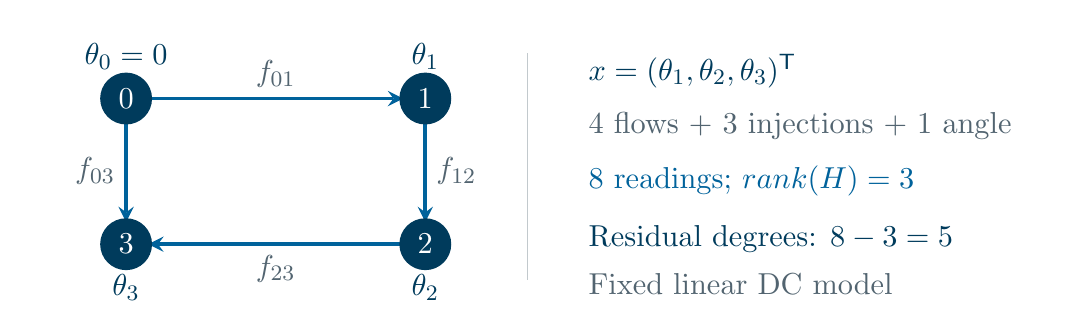
\begin{tikzpicture}[x=1cm,y=1cm,font=\fontsize{11}{13}\selectfont,>=stealth]
\definecolor{IEEEBlue}{HTML}{00629B}
\definecolor{Cyan}{HTML}{00A6B2}
\definecolor{Navy}{HTML}{003B5C}
\definecolor{Slate}{HTML}{526470}
\path[use as bounding box] (0,0) rectangle (13,3.5);
\coordinate (b0) at (1.25,2.6);
\coordinate (b1) at (5.05,2.6);
\coordinate (b2) at (5.05,.75);
\coordinate (b3) at (1.25,.75);
\draw[->,IEEEBlue,line width=1.4pt,shorten <=8pt,shorten >=8pt] (b0)--node[above,text=Slate] {$f_{01}$} (b1);
\draw[->,IEEEBlue,line width=1.4pt,shorten <=8pt,shorten >=8pt] (b1)--node[right,text=Slate] {$f_{12}$} (b2);
\draw[->,IEEEBlue,line width=1.4pt,shorten <=8pt,shorten >=8pt] (b2)--node[below,text=Slate] {$f_{23}$} (b3);
\draw[->,IEEEBlue,line width=1.4pt,shorten <=8pt,shorten >=8pt] (b0)--node[left,text=Slate] {$f_{03}$} (b3);
\foreach \n in {0,1,2,3} {\node[circle,fill=Navy,text=white,inner sep=3.5pt] at (b\n) {\n};}
\node[anchor=south,text=Navy] at (1.25,2.85) {$\theta_0=0$};
\node[anchor=south,text=Navy] at (5.05,2.85) {$\theta_1$};
\node[anchor=north,text=Navy] at (5.05,.49) {$\theta_2$};
\node[anchor=north,text=Navy] at (1.25,.49) {$\theta_3$};
\draw[Slate!35] (6.35,.3)--(6.35,3.18);
\node[anchor=west,text=Navy] at (7,2.95) {$x=(\theta_1,\theta_2,\theta_3)^\mathsf{T}$};
\node[anchor=west,text=Slate] at (7,2.25) {4 flows + 3 injections + 1 angle};
\node[anchor=west,text=IEEEBlue] at (7,1.55) {$8$ readings; $\operatorname{rank}(H)=3$};
\node[anchor=west,text=Navy] at (7,.82) {Residual degrees: $8-3=5$};
\node[anchor=west,text=Slate] at (7,.24) {Fixed linear DC model};
\end{tikzpicture}%
